%!TEX encoding = UTF-8 Unicode
% ================================================================================
\documentclass[
    fontsize=12pt,
    headings=small,
    parskip=half,           % Ersetzt manuelles Setzen von parskip/parindent.
    bibliography=totoc,
    numbers=noenddot,       % Entfernt den letzten Punkt der Kapitelnummern.
    open=any,               % Kapitel kann auf jeder Seite beginnen.
    final                   % Entfernt alle todonotes und den Entwurfstempel.
]{scrreprt}

% ===================================Praeambel==================================
%!TEX encoding = UTF-8 Unicode
%!TEX root = expose.tex

\usepackage[T1]{fontenc}
\usepackage[utf8]{inputenc}
\usepackage{microtype}      % Optimale Randausrichtung und Skalierung.
\usepackage[
    autostyle,
    ]{csquotes}             % Korrekte Anführungszeichen in der Literaturliste.
\usepackage{scrhack}        % Verhindert Warnungen mit älteren Paketen.
\usepackage[
  newcommands
]{ragged2e}                 % Verbesserte \ragged...Befehle
\PassOptionsToPackage{
  hyphens
}{url}                      % Sorgt für URL-Umbrüche in Fußzeilen u. Literatur
% }}}

% Schriftarten {{{
\usepackage{mathptmx}       % Times; modifies the default serif and math fonts
\usepackage[scaled=.92]{helvet}% modifies the sans serif font
\usepackage{courier}        % modifies the monospace font
% }}}

% Biblatex {{{
\usepackage[
    style=alphabetic,
    backend=biber,
    %backref=true
    ]{biblatex}             % Biblatex mit alphabetischem Style und biber.

\addbibresource{\jobname.bib} % Dateiname der bib-Datei.

\DeclareFieldFormat*{title}{
    \mkbibemph{#1}}         % Make titles italics
% }}}

% Dokument- und Texteinstellungen {{{
\usepackage[
    a4paper,
    margin=2.54cm,
    marginparwidth=2.0cm,
    footskip=1.0cm
    ]{geometry}             % Ersetzt 'a4wide'.
\clubpenalty=10000          % Keine Einzelzeile am Beginn eines Absatzes
                            %  (Schusterjungen).
\widowpenalty=10000         % Keine Einzelzeile am Ende eines Absatzes
\displaywidowpenalty=10000  %  (Hurenkinder).
\usepackage{floatrow}       % Zentriert alle Floats
\usepackage{ifdraft}        % Ermöglicht \ifoptionfinal{true}{false}
\pagestyle{plain}           % keine Kopfzeilen
% \sloppy                    % großzügige Formatierungsweise
\deffootnote{1em}{1em}{
  \thefootnotemark.\ }      % Verbessert Layout mehrzeiliger Fußnoten
\renewcommand*{\chapterformat}{% Hübscht Kapitelüberschrift mit senkrechtem 
	\thechapter\enskip%          grauen Balken zwischen Nummer und Text auf
	\textcolor{gray!50}{\rule[-\dp\strutbox]{2pt}{\baselineskip}}\enskip
}
%\setkomafont{disposition}{\normalcolor\bfseries} % Aus der KOMA-Skript-Anleitung: „Mit dieser Änderung verzichten Sie darauf, für alle Gliederungsebenen serifenlose Schrift voreinzustellen“

\makeatletter
\AtBeginDocument{%
    \hypersetup{%
        pdftitle = {\@title},
        pdfauthor  = \@author,
    }
}
\makeatother
% }}}

% Weitere Pakete {{{
\usepackage{graphicx}       % Einfügen von Graphiken.
\usepackage{tabu}           % Einfügen von Tabellen.
\usepackage{multirow}       % Tabellenzeilen zusammenfassen.
\usepackage{multicol}       % Tabellenspalten zusammenfassen.
\usepackage{booktabs}       % Schönere Tabellen (\toprule\midrule\bottomrule).
\usepackage[nocut]{thmbox}  % Theorembox bspw. für Angreifermodell.
\usepackage{amsmath}        % Erweiterte Handhabung mathematischer Formeln.
\usepackage{amssymb}        % Erweiterte mathematische Symbole.
\usepackage{rotating}
\usepackage[
    printonlyused
    ]{acronym}              % Abkürzungsverzeichnis
\usepackage[
    colorinlistoftodos,
    textsize=tiny,          % Notizen und TODOs - mit der todonotes.sty von
    \ifoptionfinal{disable}{}%  Benjamin Kellermann ist das Package "changebar"
    ]{todonotes}            %  bereits integriert.
\usepackage[
    breaklinks,
    hidelinks,
    pdfdisplaydoctitle,
    pdfpagemode = {UseOutlines},
    pdfpagelabels,
    ]{hyperref}             % Sprungmarken im PDF. Lädt das URL-Paket.
    \urlstyle{rm}           % Entfernt die Formattierung von URLs.
%\usepackage{breakurl}
%\def\UrlBreaks{\do\/\do-}
\usepackage{listings}       % Spezielle Umgebung für Quelltextformatierung.
    \lstset{
        language=C,
        breaklines=true,
        breakatwhitespace=true,
        frame=l,            % Linie links: l, doppelt: L
		framerule=2.5pt,    % Dicke der Linie
		rulecolor=\color{gray},% Farbe der Linie
        captionpos=b,
        xleftmargin=6ex,
        tabsize=4,
        numbers=left,
        numberstyle=\ttfamily\footnotesize,
        basicstyle=\ttfamily\footnotesize,
        keywordstyle=\bfseries\color{green!50!black},
        commentstyle=\itshape\color{magenta!90!black},
        identifierstyle=\ttfamily,
        stringstyle=\color{orange!90!black},
        showstringspaces=false,
        }
%\usepackage{filecontents}  % Direktes Einfügen von Dateiinhalt. Wird hier für
                            %  die Verwendung einer .bib-Datei in dieser .tex-
                            %  Datei benötigt.
% }}}


\renewcommand{\arraystretch}{1.5}

\addbibresource{thesis.bib}

% ===================================Dokument===================================

\begin{document}

\title{On using privacy preseving machine learning for\\decentralized web bot detection}
\author{Matz-Jona Radloff}
% \date{01.01.2015} % Falls ein bestimmtes Datum eingesetzt werden soll, einfach
                    %  diese Zeile aktivieren.


\begin{titlepage}
\begin{center}\Large
	\vfill
    Bachelor Thesis
	\vfill
	\makeatletter
	{\Large\textsf{\textbf{\@title}}\par}
	\makeatother
	\vfill
    submitted by
	\par\bigskip
	\makeatletter
	{\@author} \par
	\makeatother
	Matriculation number 6946325 \par
	Study Program: Computer Science
	\vfill
	\makeatletter
	submitted on {\@date}
	\makeatother
	\vfill
	Supervisor: August See\par
	First reviewer: Prof. Dr. Mathias Fischer \par
	Zweitgutachter: August See
\end{center}
\end{titlepage}


\chapter*{Abstract}

Malicious use of automated bots presents an increasing risk to applications in the web. Their detection represents an integral part of modern security system. Existing solutions do either not perform well, are not accessible to many providers due to high cost, or disregard modern privacy standards. This work aims to provide a proof-of-concept for a basic system that incorporates all of the above criterions. It utilizes biometric data in the form of pointer interactions.

\tableofcontents

\chapter{Introduction}

In this work, the term bot is referring to software that is automatically performing HTTP(S) requests with the intent of harming a target or reaching another malicous goal. While this threat is nothing new to the web the attack surface has grown significantly over the past years. In their yearly report, the Imperva Threat Research Lab\footnote{\url{https://www.imperva.com/blog/}} show that both the percentage of bot traffic in general and the absolute amount of malicious bot traffic have increased over time.\cite{BAD_BOT_REPORT2020,BAD_BOT_REPORT2021,BAD_BOT_REPORT2022} For example 27.7\% of 2021's internet traffic was fraudulent and automatically generate compared to 25.6\% in 2020.

The usage of bots can have several goals and can be grouped into the following categories. DoS attacks aim to overload the target's infrastructure such that it becomes inaccessible for normal use. Carding and Credential stuffing refers to performing payment or login requests to find working credit card numbers and credentials usually obtainend from a data breach. Data scrapers download the website information and can use it for malicious purposes, e.g. damage SEO or violate copyrights. Content spam includes inserting malicious or polluting data on platforms that allow user generated content. Scalping or inventory hoarding of shopping items can artificially raise prices, damage brands, generate false market forces and create a bad customer experience. Imperva's 2022 Report\cite{BAD_BOT_REPORT2022} cites Account Takeover, Scraping and Scalping as the top three most common attack types.

Most of the above attacks need to trick a webserver and their application backends into performing the request as if it had been initiated by a human. Instead of combating the resulting issues separately, bot detection could potentially mitigate many at once.

A complication in this problem space is the, often desired, requirement for non-malicious bots to be granted normal access. A prominent example are scraper bots used by search engines that need to request websites periodically to build their search indices. A common technique to exploit this requirement is trying to emulate known bot signatures from large search engines, e.g. Googlebot \cite{8421894}.

Many website operators tend to use solutions that are easy to integrate. This requires embeding external software which collects user data and sends it to servers of the software vendors. Closed source software does not allow to determine what exactly happens to the user data and website operators open themselves to additional threats in case of a data breach. Depending on the operating countries of both the websites and software vendors, data privacy regulation might also not allow sharing user data at all or require the operator to document the data transfers in a very detailed and legally complicated way. For example, in countries falling under the GDPR \cite{GDPR} a comprehensive data protection documentation is required. Because of the above reasons it is desirable to either employ self-hosted software or use a solution that does not require user data transfers.

This thesis primarily focuses on detecting web-based bots that try to access or perform actions on websites which are the primary medium with which people interact on the internet.


\chapter{Requirements and Related Work}

%\section{Proprietary Solutions}
%\url{https://datadome.co/} \\
%\url{https://www.perimeterx.com/products/bot-defender/} \\
%\url{https://www.imperva.com/products/advanced-bot-protection-management/} \\
%\url{https://www.fastly.com/products/cloud-security/bot-protection} \\
%\url{https://www.cloudflare.com/products/bot-management/} \\
%\url{https://developers.google.com/recaptcha/docs/v3} \\
%\url{https://www.hcaptcha.com/} \\

\section{Requirements}

The main requirement of a bot detection system is its performance including being reliable, having a low false positive rate and good execution speed. If these factors are degraded by including other features, this work defines the overall value still lower as without.

The most desirable additional requirement is privacy friendliness, the feasibility of which this work aims to show. For this to be met a level of transparency is required in order to comprehend the user data flow. Proprietary solutions needed to be trusted or individual agreements needed to be found.

Other optional challenges are ease of use for the operator and integration into existing solutions. These goals were be made easier if the whole or critical parts of the underlying system were available publicly and/or open-source.

\section{Related Work}

The paper of Li et al. \cite{LiJi2021} introduces a federated learning approach similar to the goals of this work but differs in the specific use case and implementation. Their system focuses on the detection of IoT (Internet of Things) devices which are easily hacked and turned into zombies. These zombies are commonly used in DDoS (Distributed Denial of Service) attacks which their strategy tries to make not feasible to perform. They also develop their own iterative model averaging based method "gated recurrent unit" (GRU) which is optimized for their specific use case.

Iliou et al. \cite{10.1145/3339252.3339267} present a comparison of different machine learning algorithms and combinations of different attributes used in previous literature. Their methods were tested on a year's worth of HTTP log data from MK-Lab's public web server\footnote{Multimedia Knowledge and Social Media Analytics Laboratory, \url{https://mklab.iti.gr/}}. The data included IP addresses, request method, request path, referrers, user agent strings and timestamps. The attributes comprise mostly of request metadata which would be suitible for a privacy-friendly bot detection system, for example the percentage of image requests or the number of total bytes per session. The authors split the bot data in their dataset into simple and advanced bots which is determined by whether the requests have a browser agent name and, in case they do, whether the IPs have shown malicious activity before. Their results show that different sets of attributes are performing best depending on the classification algorithm used. The best machine learning methods are Random Forest and Multilayer Perceptron although the paper concludes that using an ensemble classifier that averages over all used methods would be more stable. Additionally simple web bots can be detected very easily while detecting advanced bots is significantly harder, with areas under the ROC curve of $1.00$ and $0.64$ respectively. Especially in false positive intolerant use cases the performance of detecting advanced bots is too poor to be used in the real world. The authors conclude that future work would need to incorporate more advanced features which can not be easily simulated by bots.


The work of \cite{PETS2021} outlines problems and privacy-related concerns in the context of bot detection and aims to solve a very similar problem but focuses on mobile devices. They explicitely comment on and compare their work against Google's reCAPTCHA v3 \cite{RECPATCHA_V3} which is a very prevelant but opaque solution. Especially the transmission of raw user data to third party servers (which often are located in a differen country) is considered pervasive and raises privacy concerns. In their own method "zkSENSE" the authors run a pre-trained machine learning model on the users' devices such that no user data has to be sent to their or any other servers. To avoid local changes to the model a cryptographic zero-knowledge proof is generated that is verified on a server. The model iself operates on data from the mobile device's sensors including accelerometers and gyroscopes. They postulate that a human-performed touch event or click generates specific information in these sensors that is either hard to fake or absent. In a comparison of different classifier models most perform very similar with Decision Trees and Random Forest being slightly better. Finally, they also tested the performance in terms of execution time, CPU and memory utilization, and consumed bandwith with the result that their method is comparable to existing CAPTCHA solutions.


The work of Shen et al. \cite{6263955} show the viability of using mouse and trackpad actions to verify the authenticity of users. Shen et al. use a pattern-growth-based mining method in which they group raw mouse events into mouse actions, such as single click, double click or drag-and-drop. This data is combined with additional information of the current application type (e.g. surfing the internet, word processing or playing games), the screen area where the mouse movement occurred, window position and timestamp into a database of mouse operation sequences. They employ a pattern growth approach which identifies relationships within the data. The authors further state that the mined patterns cannot be used directly by a classifier and are thus converting into a feature vector containing data such as the time it took a user to click a button, movement speed or acceleration. Finally 3 different one-class detectors (Nearest Neighbor, single-layer Neural Network, Support Vector Machine) are compared resulting in the SVM method performing the best with false positive and false negative rates of 0.37\% and 1.12\% respectively. This was only achieved by incorporating 3000 operations and 30 minutes of processing for successful authentication. With a more practically feasible authentication time of one minute, the values for FPR and FNR increate to 44.65\% and 34.78\%. This drastically limits the applicability of this approach which the authors conclude as well.

Antal et al.\cite{9111596} and their previous paper \cite{https://doi.org/10.1049/iet-bmt.2018.5126} cover intrusion detection and user verification using mouse data. Their first paper analyses the Balabit dataset \cite{BALABIT_CHALLENGE}, and determines parameters for a machine learning system. The second publication also compares different datasets and explicitely mentions the bad reproducibility of previous work. The authors focussed on describing their experiments with great attention to this goal. Their approaches segment raw mouse data into mouse actions such as mouse move (MM) or mouse move and a click (point and click, PC). Multiple results are averaged to increase detection performance. Their intrusion detection system's evaluation resulted in an average accuracy of 80.17\% and an AUC value of 0.8761 when only using Balabit's training data and worse values of 72.29\% accuracy and 0.7746 AUC when additionally incorporating Balabit's test data. Their conclusion names the test data's short session length as the primary reason for the worse performance. Privacy concerns were cited as one the primary challenges of using such a methods in practice. But their good perfomance makes using mouse data a promising method if these concerns could be remedied.

Acien et al. \cite{Acien2020BeCAPTCHAMouseSM} show the feasibility of using biometric features for bot detection. They use both function-based and GAN-based mouse trajectory synthesis methods to generate training and evaluation data. Six different classifier types (Support Vector Machine, K-Nearest Neighbor, Random Forest, Multi-Layer Perceptron and 2 Recurrent Neural Networks with Long Short-Term Memory and Gated Recurrent Units respectively) are compared to each other with Random Forest performing the best. Combined their method can distinguish between humans and bots with up to 98.7\% accuracy with only one mouse trajectory as input. They conclude that, compared to state-of-the-art works, the usage of mouse data has unexploited potential in the context of bot detection. Their "BeCAPTCHA-Mouse Benchmark" data and implementations are unfortunately not available publicly.

In their 2004 paper, Pusara et al. \cite{10.1145/1029208.1029210} use mouse movement data to re-authenticate already logged in users with the goal of identifying anomalous behavior to combat insider attacks where a potential assailant might have access to an existing user session. Similar to Antal et al.'s \cite{https://doi.org/10.1049/iet-bmt.2018.5126} extracted features, the authors use both the raw mouse events and derivative data, such as angle speed, distance as well as values for the mean, standard deviation and third moment over multiple samples. Decision tree classifiers and a smoothing filter were used to reach average false positive and false negative rates of 0.43\% and 1.75\%, although with high variability depending on which concrete users were used as input. While these initial results are promising, the authors conclude that scalability might become an issue as their model needs to be trained for each combination of users. As this approach requires already logged in users and is designed to identitfy specific users only its application in the context of bot detection is limited but the successful usage of mouse data is shown.

% file:///Z:/uni/thesis/papers/mouse_feature_papers/A_New_Biometric_Technology_Based_on_Mouse_Dynamics.pdf
Ahmed et al. pursue the very similar goal of identifying users based on mouse dynamics. In an own experiment they collected 998 session of 22 participants
A MLP-based neural network with a single hidden layer of 40 neurons was used for classification. The raw data was segmented into the mouse actions types mouse-move, drag-and-drop, point-and-click and silence. Together with the corresponding distance in pixels, time, speed and direction (8 directions spanning $45\deg$) this data was passed through a noise reduction stage, followed by inputting it into the neural network. The authors conclude that, despite their results' good false positive and false negative rates of 2.4649\% and 2.4614\%, practically viable access control was not achieved. Despite this the values were still better than some established methods based on biometric data, e.g. voice or face recognition.

\todo{maybe more }

\chapter{Method}

The thesis explores how biometric data can potentially improve a machine learning system for bot detection. Compared to data that is only indirectly generated by a human, for example web requests metadata, biometric data contains more information that can be directly used to decide whether a bot or human generated the data. A big part of request data is redundant as it either does not change between different requests or clients, e.g. the "User-Agent" header, or can be easily faked. Illustrated by figure \ref{fig:user_mouse_heatmap}, human-generated mouse data contains many different movements which are hard to model for an attacker.

\begin{figure}[h]
	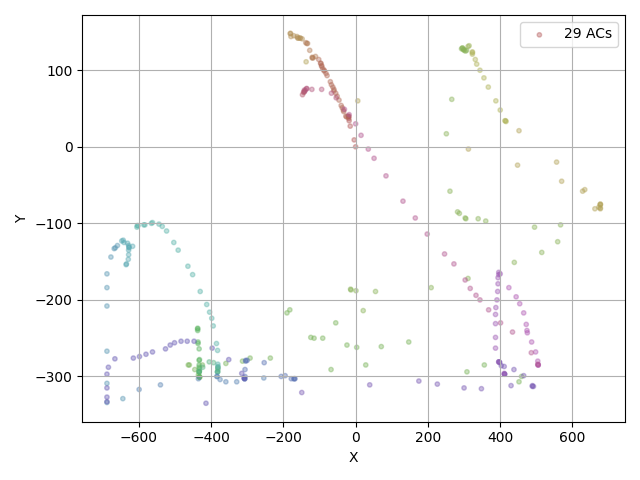
\includegraphics[width=\textwidth]{figures/user_mouse_heatmap.png}
	\caption{29 Mouse movements captured from a human user}
	\label{fig:user_mouse_heatmap}
\end{figure}

As previous works showed, mouse data in combination with machine learning systems have the potential to perform well enough for practical use but lacked either performance or execution speed, especially when trying to differenciate between different human users. When reducing the goal to only detecting bots versus any human, this work aims to show the increased viability. Its approach differs from similar works, such as Acien et al.'s BeCAPTCHA method \cite{Acien2020BeCAPTCHAMouseSM} in that it also hypothesises that a simplified approach in terms of model parameters, input feature complexity can be found to improve the practical feasibility, ease of deployment and execution speed. This is achieved by performing both the experiments and data collection as well as the evaluation in an environment which is representative of a real application.


\section{Concept}

For classification a system based on machine learning is chosen because it allows learned knowledge about different bot behavior to be more easily transfered between systems without compromising user privacy in comparison to other methods. For example federated learning \cite{DBLP:journals/corr/KonecnyMR15} \cite{DBLP:journals/corr/KonecnyMRR16} is an approach that only shares internal model parameters which are sufficiently anonymized so that specific users cannot be identified. It consequently allows the incorporation of very sensitive personal data which, this work hypothesizes, will improve the performance. Compared to the often very artificially constructed environments of related works, this thesis tries to use a very realistic and web-based approach.

A similar system to the proposed architecture of Iliou et al. \cite{10.1145/3339252.3339267} is implemented for detecting bots via request data. Their work is used as the basis for the machine learning system to compare against. They evaluated the most promising features that have been proposed over 5 years prior to their publication (2019) and accumulated their findings in concise results.

Mouse, touchpad or touch gestures (pointer data) are used as the second type of data in this work's approach. This data is harder to fake by attackers trying to emulate human behavior. Because it would be classified as sensitive user data, this type of data collection and processing could not reasonably be used by a third party provider or without a strictly necessary reason and would require explicit user consent \cite{GDPR}. Thus it would be best to process the data in an anonymized and indirect way which this method of machine learning provides as well. Derived data features are adapted from previous works and limited to simplify the preprocessing while maintaining good performance.

It is also shown that the requirement of good execution speed is met by integrating the trained model into the experiments' websites as representative real-world applications. As the recorded data is aggregated over time per user, each server response includes the current score as a number between 0 and 1. How much of the past data can be used without compromising request performance is additionally determined.

\section{Datasets}

To realistically match request metadata and user mouse data a dataset is gathered from two websites in a user experiment. This way biases of different datasets are eliminated and the different systems' performances can be directly compared against.

The websites have a basic blog-style structure with different information sections and user registration features. Their web servers log all relevant data to extract the features required for the request data approach while a javascript library records mouse data and sends it to the site's backends for storage.

To verify the proposed system does not overfit to the experiment's limited data, different public data is used to compare against. While no suitible datasets exist that include both request and mouse data, datasets that contain real-world user mouse movement and interaction data are publicly available.

The Balabit Mouse Dynamics Challenge dataset \cite{BALABIT_CHALLENGE} includes a few longer and several shorter sessions which are meant to be used for training and testing respectively.
Antal et. al's dataset \cite{9111596} includes 21 users with around 20-30 sessions each. Their work compares their own dataset against the Balabit and ChaoShen datasets. In their scenario of detecting whether mouse data belongs to a specific user, the former corresponds to better but comparable results.
At the time of publication the referenced ChaoShen dataset is not available anymore.

Antal et. al's dataset is used to validate the transferability of this method because of its better performance and because the other datasets are older and have been used more in other publications.


\section{Machine Learning Model}

Many different machine learning models are suitable for binary classification. Hu et al. \cite{8275816} compare different classifiers in a context where mouse data is used. Random Forest and Multilayer Perceptron (MLP) perform the best.
Iliou et al. \cite{10.1145/3339252.3339267} also show that Random Forest and MLP perform well when using request metadata.

Random Forest\cite{Breiman2001} is a perturb-and-combine technique that uses an ensemble of decision trees. Decision tree learning in general is a supervised machine learning method which can be used for classification or regression depending on the output being a discrete value (i.e. class) or real number. For each node of the tree a binary decision criterion is calculated and the data is split accordingly. With increasing tree depth this approach is able to approximate very irregular models but also has a high risk of overfitting. Random Forests extend this technique by randomizing the input sample selection and parameters with the goal of decreasing the variance and avoiding overfitting. Choosing a random subset of inputs repeatedly is generally known as bootstrap  aggregation or bagging. The Random Forest algorithm in particular additionally randomizes the input selection at each node when growing the tree to further increase the resulting benefits. The final prediction is calculated from the average over all trees. The used implementation's documentation notes that compared to the original publication, their method averages over the probabilistic predictions, instead of only single decisions.\footnote{\url{https://scikit-learn.org/stable/modules/ensemble.html\#random-forests}} Their decision trees' used split criterion function is the Gini impurity which compares the amount of incorrect labeling of randomly chosen samples if their label (for the current feature) was also chosen randomly to the currently assigned label.

Multilayer Perceptron describes a type of feedforward artificial neural network which connects many perceptron algorithm instances. It is inspired by biological neural networks and has at least three layers (input, hidden, output) which are usually fully connected. By iterating over training data, values for the perceptron's weighted inputs are learned such that the overall system behaves as a classifier or system for regression analysis.

As their performance is comparable in this context and Random Forest's implementation is easier as well as more performant compared to MLP, the former is chosen for this work.

\subsection{Model Parameters}

The most important parameters of the Random Forest algorithm are the number of estimators (i.e. number of decision trees) and the maximum number of randomly selected features per estimator. In general as more trees are used less overfitting occurs and the model generalizes better. \todo
% https://en.wikipedia.org/wiki/Random_forest#cite_note-elemstatlearn-3
% https://hastie.su.domains/ElemStatLearn/

Additional parameters include the minimum number (or fraction) of samples required to split a node ($min_samples_split$). When using the minimum value of two, node splitting is effectively unrestricted. Bigger values also affect the maximum tree depth. It can either be set directly as a parameter or is the depth at which all leaves contain no more than $min_samples_split$ samples. In the unrestricted case, this means that all leaves need to be pure when the maximum depth is reached. Additionally weights can be assigned to different classes or samples. For binary classification class weights are not considered and sample weights might be useful if there is additional data available before classification. When combining this type of machine learning system with other bot detection systems, their existing prediction could be added as weights. As this thesis only considers the classifier itself, no weights are used. Finally the maxmimum number of features that are tested when determining the node split can be set. Scikit-learn's implementation \footnote{\url{https://scikit-learn.org/stable/modules/generated/sklearn.ensemble.RandomForestClassifier.html}} uses the square root of the total feature count which is also recommended by previous literature. \cite{Hastie2009}

An empirical search is used to determine the best parameters for this use case. Additionally it is evaluated how the predictive performance changes for different amounts of training data.

\subsection{Feature Selection}

The following sections describe for both request and mouse data which features are chosen and how they are used as inputs for the Random Forest machine learning system. Previous works are referenced which already compared several different possiblities in similar contexts.

\subsubsection{Request Data}

Iliou et al. \cite{10.1145/3339252.3339267} ranked the best performing metrics for simple and advanced bots per classification algorithm. For Random Forest, some attributes are not suitible in this theses. For example the authors include a boolean indicating whether a request has a known search engine in their "Referer" header (attribute 14). Because participants are asked to visit the websites directly this attribute is omitted. The websites are otherwise designed such that all of the above attributes are meaningful. The used attributes are listed in the implementation section.

The following selection from Iliou et al.' work \cite{10.1145/3339252.3339267} is used.

\begin{enumerate}
	\item The percentage of HTTP requests that led to an HTTP 4xx code response. (7)
	\item The percentage of HTTP requests that requested a css file. (10)
	\item The percentage of HTTP requests that requested a JavaScript file. (11)
	\item The percentage of HTTP requested URLs that contain the previously requested URL as a subpart. (20)
	\item The total time (in seconds) between the first and the last HTTP request of the session. (21)
	\item Standard deviation of requested pages' depth (i.e. number of ’/’ in URL path).
\end{enumerate}

\label{concept_mouse_data}
\subsubsection{Mouse Data}

The mouse data features consist of the (normalized) $x$- and $y$-coordinates as well as a time value for each mouse event. Additional features are engineered similar to Gamboa et.al.\cite{GAMBOA2004} and \cite{https://doi.org/10.1049/iet-bmt.2018.5126}, including the path length from the origin, angle of the path tangent, horizontal, vertical and overall velocity, acceleration, jerk, angular velocity. Additionally the type of action, length of the movement and time needed to complete the action will be used. Some features used in the authors' work have been omitted with the goal of simplifying and speeding up the feature extraction which can be revisited if the performance seems poor.

Single mouse data points are grouped based on the following rules: They either end with a click, have a maximum of 50 data points or span a maximum of two seconds. The features are calculated for each group. As a basis for all derived values, the time, x and y coordinates are linearly interpolated such that vectors with uniformly spaced values $x'_t$ and $y'_t$ every $20ms$ are generated. All inidices start at zero.

The path length from the origin $s_t'$ is the accumulated sum of previous segment lengths:

\[
s'_t = \sum_{k = 0}^{t - 1} \sqrt{(x'_{k+1} - x'_{k})^2 + (y'_{k+1} - y'_{k})^2}
\]

The angle of the path tangent with the x-axis $\theta_t$ is the arctangent ($atan2$ is used, which returns only values $-\pi < \theta < \pi$) of the segment at time $t > 0$. At $t=0$ an angle of $0$ is assumed.

\[
\theta_t = atan2( (y'_{t+1} - y'_{t}), (x'_{t+1} - x'_{t}) )
\]

The temporal features horizontal ($v_x$), vertical ($v_y$), tangential ($v$) and angular velocity ($\omega$) as well as tangential acceleration ($\dot{v}$) and jerk ($\ddot{v}$) are computed as follows:

\[
v_x = \frac{\delta x}{\delta t}; \quad
v_y = \frac{\delta y}{\delta t}; \quad
v = \sqrt{v_x^2 + v_y^2}; \quad
\omega = \frac{\delta \theta}{\delta t}; \quad
\dot{v} = \frac{\delta v}{\delta t}; \quad
\ddot{v} = \frac{\delta \dot{v}}{\delta t}
\]

For each of the $9$ vectors ($x'_t$, $y'_t$, $s'_t$, $v_x$, $v_y$, $v$, $\omega$, $\dot{v}$, $\ddot{v}$) the mean, standard deviation, minimum, maximum and value range (max - min) yield the first $45$ feature values.

Additionally the time $t_total$ and length $s_{n-1}$ of the stroke (i.e. group of $n$ data points), its straightness and jitter are computed. The time is the difference between the first and last datapoints' timestamps and the length can is the accumulated sum of segment lengths but using the raw instead of the interpolated data.

\[
t_{total} = t_{n-1} - t_0
\]

\[
s_{n-1} = \sum_{k = 0}^{n - 1} \sqrt{(x'_{k+1} - x'_{k})^2 + (y'_{k+1} - y'_{k})^2}
\]

Analogous to Gamboa et.al.'s definition\cite{GAMBOA2004} the straightness is defined as the ratio of the Euclidian distance between the first and last points of each group, and the total distance:

\[
straightness = \frac{ \sqrt{ (x_0 - x_{n-1})^2 + (y_0 - y_{n-1})^2 } }{s_{n-1}}
\]

The jitter is the ratio between the original and smoothed path lengths:

\[
jitter = \frac{s'_{n'-1}}{s_{n-1}}
\]



\subsection{Classification and Evaluation}

The actual classification is performed by splitting the extracted features into training and test data. The partitions contain 90 and 10 percent of the data, respectively, with each data entry being assigned randomly. The training data also includes the "is bot" label which the model uses to calculate its error while learning. In the testing phase a predicted label is compared to the known value. The fraction of correct over the total number of predictions, i.e. accuracy is used as the primary evaluation metric. Additionally the False Positive Rate (FPR) and False Negative Rate (FNR) are computed which are the fraction of wrong guesses. The False Positive Rate is weighed higher because a prediction that a user is a bot has a qualitatively much greater impact than the opposite case. Plotting one against the other results in a Receiver operating characteristic (ROC) curve. The area below this curve (AUC) is another metric used for comparing results because it provides a single and condensed numerical value. When using normalized units, its concrete value represents the probability that the model will perform better when given a randomly selected positive and negative sample.\cite{FAWCETT2006861}

\section{Experiment/Data Collection}

A user experiment was announced to all members of the University of Hamburg to gather a representative dataset for human interactions on websites. The specific goal of the experiment was not directly included in the announcement to avoid any biases as much as possible. To gather all required data a custom website with two different frontend layouts and designs was implemented.

\subsection{Websites}

The structure and content mimic blog-style websites with login and register functionalities. They contain a landing page, an about page with additional information about the experiment and this thesis and a contact / imprint page. On first visit users get presented a dialog asking to confirm the data collection. After registering or logging in a profile page is accessible where basic user information can be added or edited. The main part of both websites is a blog section containing randomly generated entries which can be viewed on an overview page or on detail pages which only show a single entry.
All parts give opportunity for user input, similar to regular websites including many possible navigation paths and form interactions.

One difficulty of recording both request and mouse data is that the former benefits from having as many requests per interaction as possible while full page reloads would restart the mouse data collection and might lose data. Usually websites would decide between a traditional approach, where URL changes would load a completely new page and fulfill the former requirement, and a SPA (Single Page Application) where only parts of the content are changed dynamically by JavaScript implementations which would allow mouse events to be recorded continuously.

To combine the advantages of both approaches a hybrid system is used that intercepts URL changes, e.g. from clicking a link, preventing the default action and loading the target page through a separate HTTP request. The main content section is then replaced by the newly loaded HTML data. From the backend's point of view at least one request is performed per visited page while mouse data is recorded without any gaps.

All users, logged in or not, are identified by a version 4 UUID which is immediately stored in cookie after accepting the initial dialog prompt. Every data point that is written to the database gets a reference to the correspoding user and the current date and time.

\subsection{Request Metadata}

For the request metadata relevant information of every request is recorded. Flask allows to register functions which are called at specific points in the request lifecycle. For this purpose the \lstinline{after_request} decorator is used which is called right before the handled request is returned.

Bot data is generated by sending requests to the same websites but including an additional query string which details the current bot configuration.

The following data is stored in the database:

\begin{table}[]
\begin{tabular}{|l|l|}
\hline
user uuid & The current user's UUIDv4 \\ \hline
request method & One of \{'GET', 'POST'\}, other request methods are not used \\ \hline
request url & The full request URL including \\ & scheme, host, root path, path and query string \\ \hline
request path & The request path \\ \hline
request origin & The host from which the request was sent from \\ \hline
request remote address & The IP address of the client \\ \hline
request referrer & The referer value from the corresponding header field \\ \hline
response content type & The response's body media type \\ \hline
response content length & The response's body size in bytes \\ \hline
response date & The date and time of the response \\ \hline
response status code & The HTTP status code of the response \\ \hline
user type & One of {Bot, Human} \\ \hline
random delays & Whether random delays for bot-generated requests were enabled \\ \hline
advanced & Whether the advanced bot version was used \\ \hline
bot mode & One of \{Request, Mouse\} \\ \hline
data type & One of \{Request, Mouse\} \\ & saved separately because e.g. mouse bots also generate request data \\ \hline

\end{tabular}
\end{table}

\subsection{Mouse Data}

All information for the mouse datasets is recorded by a JavaScript library which is deployed as part of a VueJS application. It registers listener functions for the events \lstinline{pointermove, pointerdown, pointerup} on the whole document which are throttled to $30$ events per second. Pointer events are used because they include mouse, touch, pen/stylus and other pointing devices. For every event the following data is recorded:

\begin{table}[]
\begin{tabular}{|l|l|}
\hline
user uuid & The current user's UUIDv4 \\ \hline
type & One of \{'pointermove', 'pointerdown', 'pointerup'\} \\ \hline
position & The pointer's x and y screen coordinate in pixels \\ \hline
document size & The document's width and height in pixels \\ \hline
pointer type & One of \{'mouse', 'pen', 'touch'\} \\ \hline
buttons & What buttons are pressed as a binary encoded integer \\ \hline
dt & The date and time of when the event occurred \\ \hline

\end{tabular}
\end{table}

All events are cached locally in a list which is sent to the backend every two seconds which writes every data point individually to the database. This request is excluded from the request data capture.

\section{Bot Data Generation}

To generate bot data the different variants were implemented by using the selenium-python and puppeteer (JavaScript) libraries.\footnote{\url{https://selenium-python.readthedocs.io/}} \footnote{\url{https://pptr.dev/}} They are designed to run automated actions in a browser environment.

Most bot variants were implemented as a generic class \lstinline{Bot} which sets up a selenium webdriver instance and provides wrapper methods for randomly waiting between calls and locating elements. When instantiated it starts a  browser instance with a specific window size. Firefox was used as the browser backend and 1366x768, 1920x1080 and 2560x1440 were used as the window sizes as these represent very common monitor resolutions.\footnote{\url{https://gs.statcounter.com/screen-resolution-stats/desktop/worldwide}} The class also handles the initially required request to set the current bot parameters and saves the returned cookie. The advanced mouse bot was implemented separately with puppeteer and the extension ghost-cursor \footnote{\url{https://github.com/Xetera/ghost-cursor}} because many instances could be run in parallel. After initially planning to use the PyAutoGUI \footnote{\url{https://pyautogui.readthedocs.io/en/latest/}} library, it turned out that its method of faking a cursor was not compatible with running headless browser instances without GUIs. The puppeteer automation was otherwise implemented to have the exact same methods as the selenium variant.

The classes \lstinline{RequestBot} and \lstinline{MouseBot} inherit from \lstinline{Bot} and implement methods for the following actions:

\begin{enumerate}
	\item Accepting the initial prompt dialog to start the experiment
	\item Visiting the top-level pages \{About, Blog, Contact/Imprint, Login, Register\}
	\item Visiting 10 randomly selected single blog pages with a parameter for how many
	\item Visiting 100 completely randomly selected pages with a parameter for how many
	\item Registering an account
	% \item Filling in profile data
\end{enumerate}

Randomly choosing the next link to click in action 3. and 4. increases the data's variance greatly by allowing for many different combinations of start and end points for mouse movements.

All actions are configued to wait for the target element to be visible and clickable, scrolling it into view, if not. If configured as such, before each action a random delay between $0$ and $2$ seconds is waited for.

The request bot primarily uses selenium's basic \lstinline{click}, \lstinline{back} and \lstinline{send_keys} methods to perform the actions. Barring the random delays it will perform the actions as fast as possible.

% \subsection{Mouse Bot}

The mouse bot uses the same Selenium-based methods for locating elements but replaces the basic actions with Selenium's ActionChains which can automate low-level interactions including mouse movements, mouse button actions and keypresses. By default it interpolates linearly between the starting and ending locations of the movement. Ghost-cursor's implementation uses bezier curves with randomly selected control points in a limited area on one side of the line between start and end points. Additionally the specific move and click coordinates are also selected randomly from the target element's area. Figure \ref{fig:bot_mouse_heatmap} visualizes the generated mouse movements from one bot session.


\begin{figure}[h]
	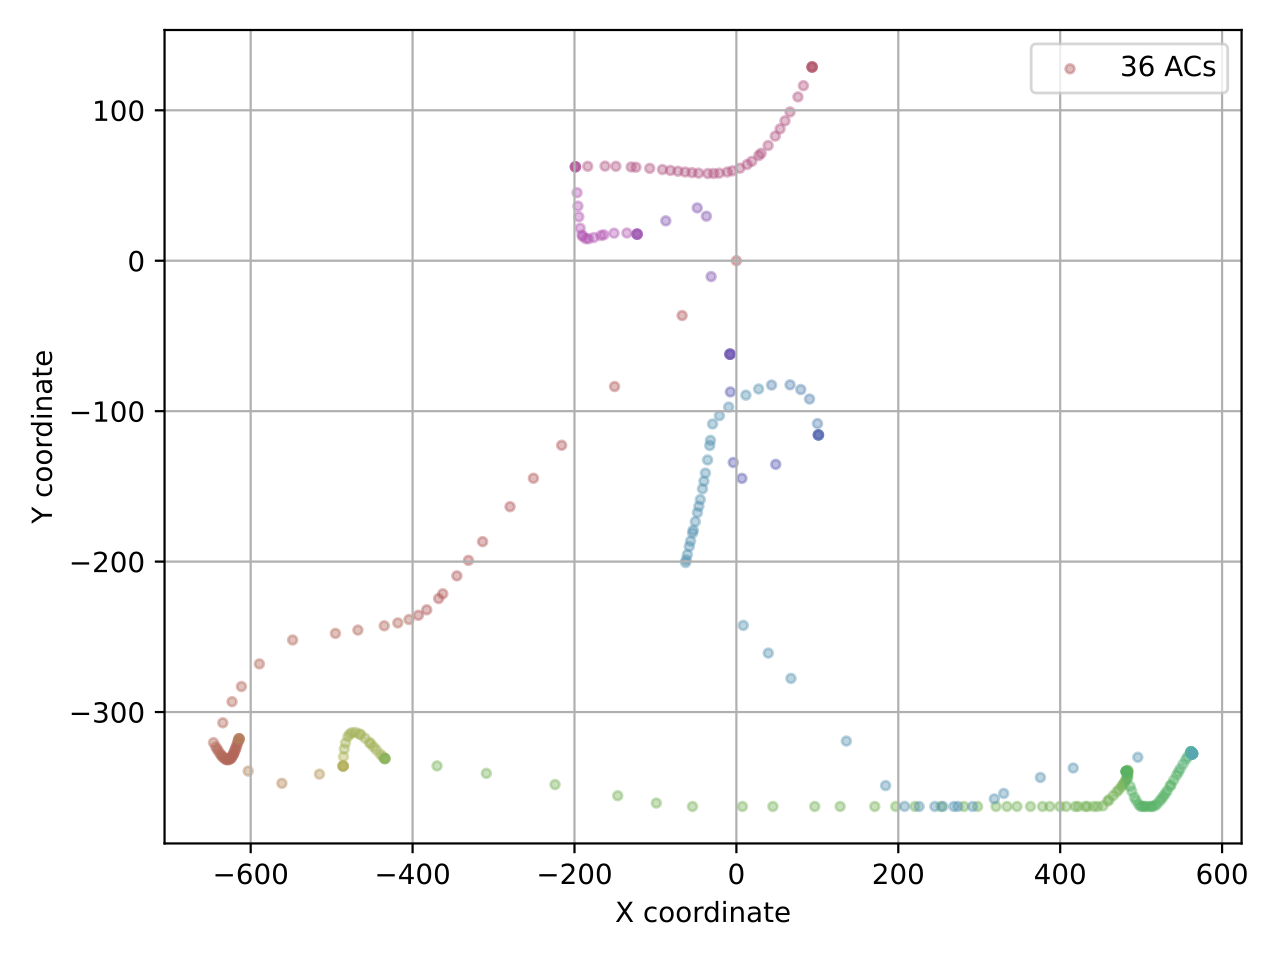
\includegraphics[width=\textwidth]{figures/bot_mouse_heatmap.png}
	\caption{Advanced Bot Mouse Movements Example}
	\label{fig:bot_mouse_heatmap}
\end{figure}



\section{Implementation}

The basis of the experiment's websites is a Flask\footnote{\url{https://flask.palletsprojects.com/}}-based python application. They are deployed behind a nginx reverse proxy web server which exposes them on two public domains. All web and application servers run on a bare-metal linux computer located in a German datacenter and are configured as real applications would be in a production environment. A postgresql server with two separate databases is also deployed. For evaluation their data was mirrored to local postgresql instances and queried directly from the same python application that runs the websites to avoid code duplication and benefit from SQLs expressiveness.

\subsection{Feature Extraction}

First, the stored unique users are filtered based on a minimum number of data points (20). In a (multi-threaded) pre-processing step the feature data is queried, loaded and calculated per user and labeled as "human" or "bot".

The request data is aggregated per user and the features are calculated as described in the \nameref{concept_mouse_data} section.

The mouse data is also calculated per user but grouped into actions. Each action represents a mouse movement that is either a maximum of $2$ seconds long or ends with a click. It is also ensured that within any action the screen resolution or page scroll position does not change.

\subsection{Evaluation}

For training and classification the implementation uses the RandomForestClassifier class from the scikit-learn\footnote{\url{https://scikit-learn.org/stable/}} library. The standard methods $fit$, $score$ and $predict$ are used to train the model and test its accuracy. Additional metrics are calculated using custom methods. Classes and launch scripts are implemented for bot data generation, loading the external dataset and generating figures for visualization.


\chapter{Evaluation}

\section{Experiment Data Quality}

The experiment assumed that participants use the provided website frontends which set cookies to map recorded datapoints to specific users. The first website's basic statistics showed that 124867 unique users have been recorded which indicates that an actual bot was used to visit this website which did not execute Javascript and set the cookie correctly. The histogram of the number of datapoints per users confirms that the vast majority of users only map 0-1 datapoints. With the chosen threshold of 2 datapoints per user the experiment resulted in recording 321 and 240 participants respectively. Figure \ref{fig:user_dp_hist} shows the distribution of the number of user (request and mouse) in terms of the number of datapoints.

\begin{figure}[h]
	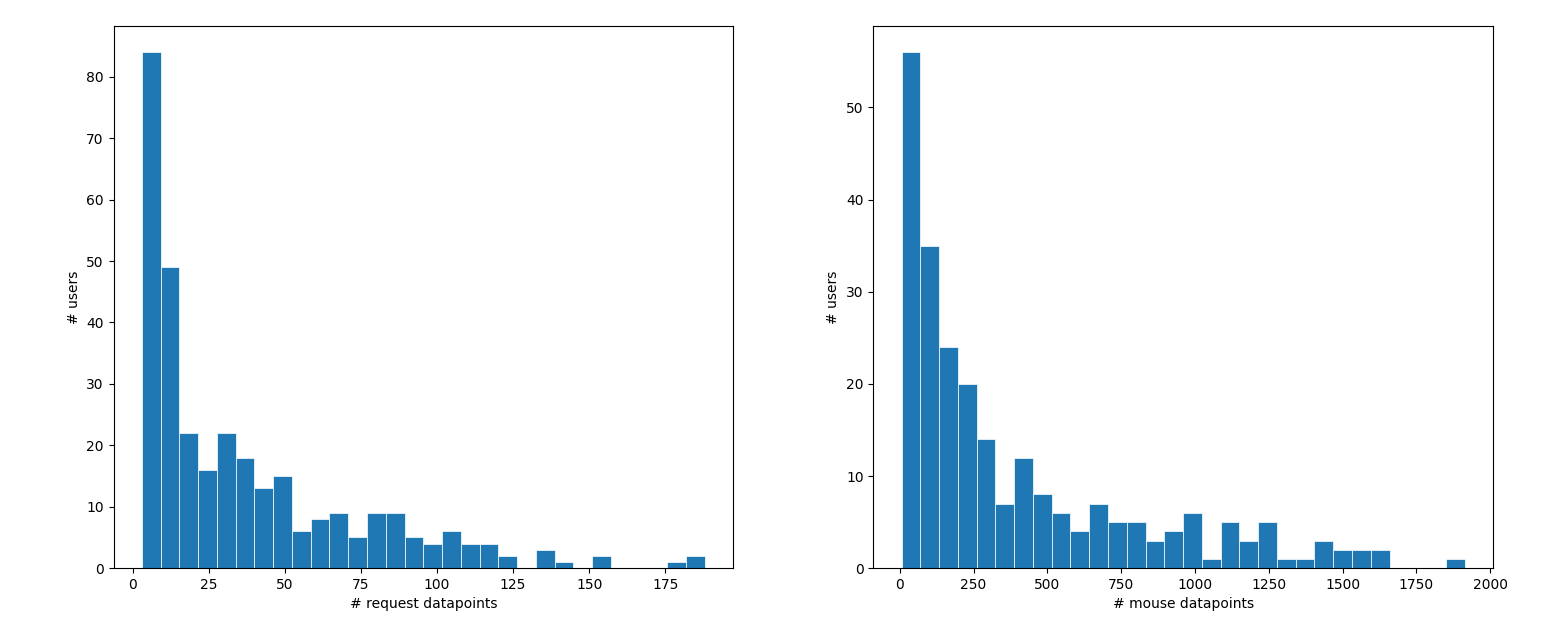
\includegraphics[width=\textwidth]{figures/user_dp_hist.png}
	\caption{Distribution of users in terms of datapoint count}
	\label{fig:user_dp_hist}
\end{figure}


\section{Model Hyperparameters}

To empirically determine the best Random Forest parameters both mouse and request data (not advanced, with random delays) from the experiment's first website and generated bots (same number of sessions as human users) were used to calculate the accuracy for combinations of the following parameters:

\begin{enumerate}
	\item Number of estimators (10, 50, 100, 150, 200, 1000)
	\item Maximum number of features (None, log2, sqrt)
	\item Maximum tree depth (None, 1, 2, 3, 4)
\end{enumerate}

Table \ref{table:mouse_params} and \ref{table:request_params} show the $16$ best performing combinations for mouse  and request data.

\setlength{\arrayrulewidth}{0.2mm}
\setlength{\tabcolsep}{18pt}
\renewcommand{\arraystretch}{0.9}


\begin{table}[h!]
\centering
\caption{Model accuracy for different parameters (mouse data)}
\label{table:mouse_params}
\begin{tabular}{|l|l|l|l|l}
\hline
Max\_features' & 'n\_estimators' & 'max\_depth' & Accuracy \\
\hline
None          & $ 10$           & None         & $ 0.9975874547647768$ \\
sqrt          & $ 200$          & None         & $ 0.9951749095295537$ \\
None          & $ 100$          & None         & $ 0.9951749095295537$ \\
sqrt          & $ 10$           & None         & $ 0.9939686369119421$ \\
None          & $ 50$           & None         & $ 0.9939686369119421$ \\
None          & $ 1000$         & None         & $ 0.9939686369119421$ \\
sqrt          & $ 50$           & None         & $ 0.9927623642943305$ \\
sqrt          & $ 150$          & None         & $ 0.9927623642943305$ \\
sqrt          & $ 1000$         & None         & $ 0.9927623642943305$ \\
sqrt          & $ 100$          & None         & $ 0.9927623642943305$ \\
None          & $ 200$          & None         & $ 0.9927623642943305$ \\
None          & $ 150$          & None         & $ 0.9927623642943305$ \\
None          & $ 1000$         & $ 4$         & $ 0.9927623642943305$ \\
None          & $ 10$           & $ 4$         & $ 0.9927623642943305$ \\
log2          & $ 50$           & None         & $ 0.991556091676719$ \\
log2          & $ 200$          & $ 0$         & $ 0.991556091676719$ \\
\hline
\end{tabular}
\end{table}

\begin{table}[h!]
\centering
\caption{Model accuracy for different parameters (request data)}
\label{table:request_params}
\begin{tabular}{|l|l|l|l|l}
\hline
Max\_features' & 'n\_estimators' & 'max\_depth' & Accuracy \\
\hline
sqrt & $ 200$  & None & $ 0.8723404255319149$  \\
sqrt & $ 150$  & None & $ 0.8723404255319149$  \\
sqrt & $ 1000$ & None & $ 0.8723404255319149$  \\
log2 & $ 200$  & None & $ 0.8723404255319149$  \\
log2 & $ 150$  & None & $ 0.8723404255319149$  \\
log2 & $ 1000$ & None & $ 0.8723404255319149$  \\
sqrt & $ 50$   & None & $ 0.851063829787234$   \\
sqrt & $ 100$  & None & $ 0.851063829787234$   \\
None   & $ 50$   & None & $ 0.851063829787234$   \\
log2 & $ 50$   & None & $ 0.851063829787234$   \\
log2 & $ 100$  & None & $ 0.851063829787234$   \\
sqrt & $ 10$   & None & $ 0.8297872340425532$  \\
None   & $ 200$  & None & $ 0.8297872340425532$  \\
None   & $ 150$  & None & $ 0.8297872340425532$  \\
None   & $ 1000$ & None & $ 0.8297872340425532$  \\
None   & $ 100$  & None & $ 0.8297872340425532$ \\

\hline
\end{tabular}
\end{table}


\section{Request Data Performance}

\todo{more text+explanation}

To match the number of users, the same number of bots with variable session length is compared against.

The model's accuracy when only using the request-type data points is $76.60\%$ and $76.92\%$ for the two websites recpectively which indicates that this performance might be a limitation of the model. Their ROC curves \ref{fig:roc_request_both_instances} show that \todo{generate more bot data}.

\begin{figure}[h]
	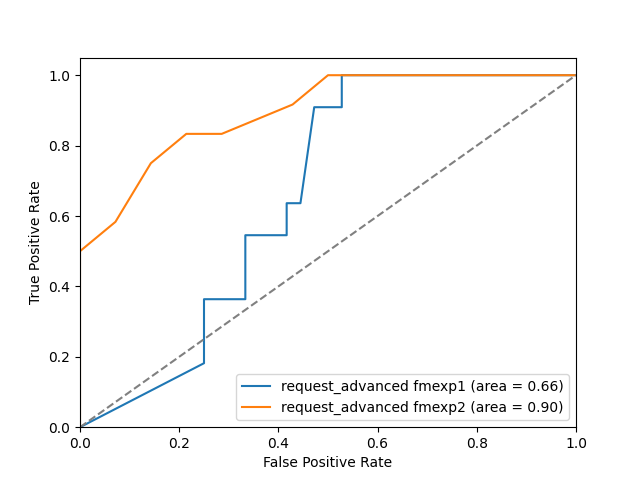
\includegraphics[width=\textwidth]{figures/roc_request_both_instances.png}
	\caption{Distribution of users in terms of datapoint count}
	\label{fig:roc_request_both_instances}
\end{figure}


\section{Mouse Data Performance}

\todo{TP FP table, different experiments}

When using mouse data, the classifiers' accuracies are $95.66\%$ and $93.58\%$ which is significantly better compared to using only request data and confirms the hypothesis that bot detection works better when incorporating biometric data. Their ROC curves \ref{fig:roc_mouse_both_instances} show that the requirement for a low False Positive Rate is also met. Their areas under the curve of $0.98$ also show this methods good performance.

\begin{figure}[h]
	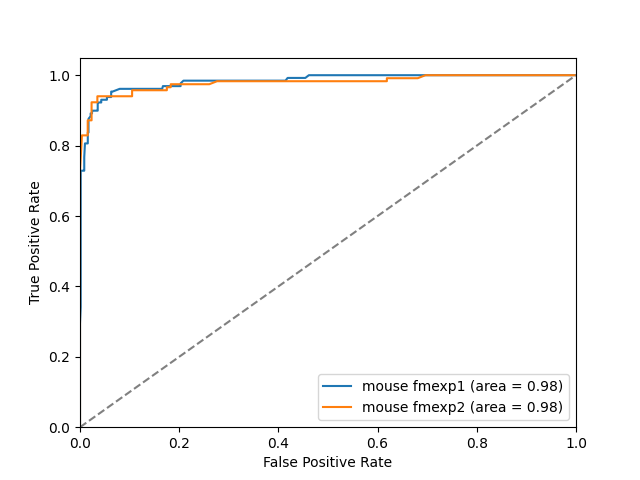
\includegraphics[width=\textwidth]{figures/roc_mouse_both_instances.png}
	\caption{Distribution of users in terms of datapoint count}
	\label{fig:roc_mouse_both_instances}
\end{figure}

\section{Performance on External Dataset}

\todo{more text}

To compare the performance to different real-world data, Antal et. al's dataset \cite{9111596} is used. Their raw mouse movement and interaction data is preprocessed in the same way as the experiment's data. This results in a much larger test set. For example "User1"'s 31 session files include $2.6M$ raw datapoints which are integrated into $64k$ input vectors.

For comparison the model is trained on data from each instance and both combined. When scoring the model with "User1"'s data as the test set, the model's accuracy increases to $99.11\%$, $99.05\%$ and \todo. For the whole dataset, which resulted in $1.54M$ input vectors, the accuracy dropped to $98.20\%$, $97.94\%$.

\begin{figure}[h]
	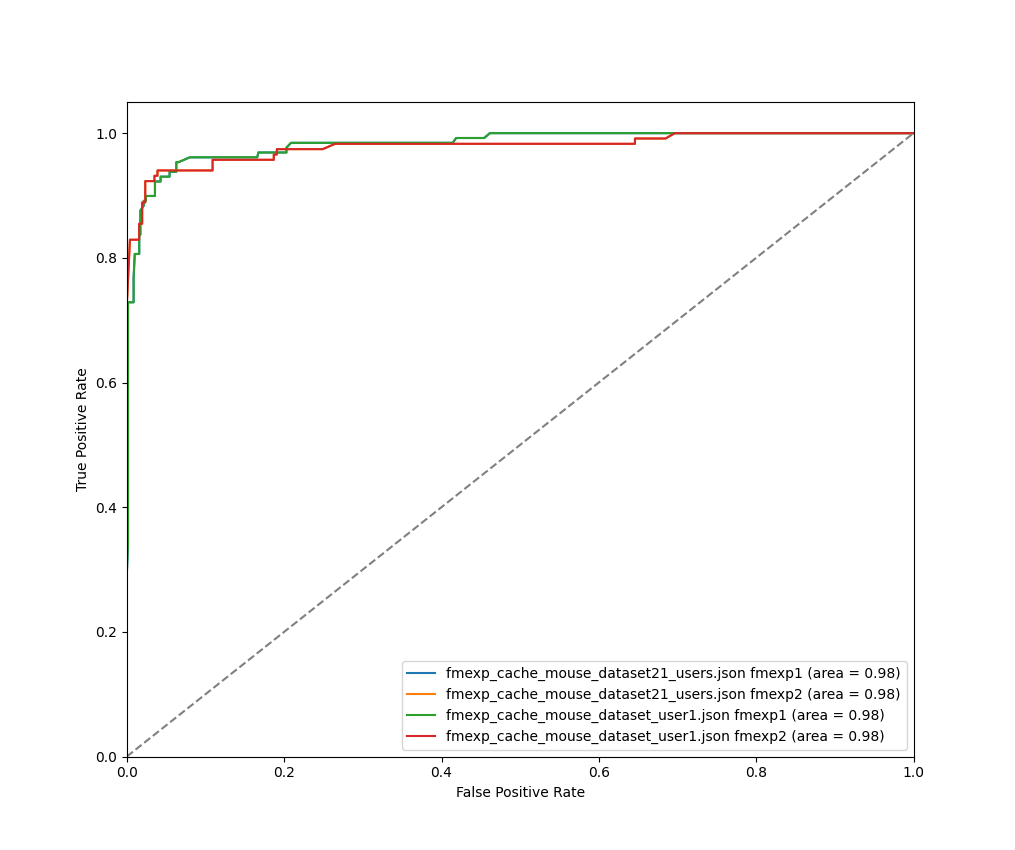
\includegraphics[width=\textwidth]{figures/roc_both_datasets_both_instances.png}
	\caption{ROC curves}
	\label{fig:roc_both_datasets_both_instances}
\end{figure}


\section{Execution Speed Performance}

The execution speed is measured by predicting a score after each request. The total time, time without extracting the features and score are logged and averaged over multiple requests. These values are calculated for different amounts of previous data points which are incorporated. This is significant because the mouse features include many values which are accumulated over many data points. \ref{fig:speed_per_dp_count} shows the times and performance for the different numbers.

\begin{figure}[h]
	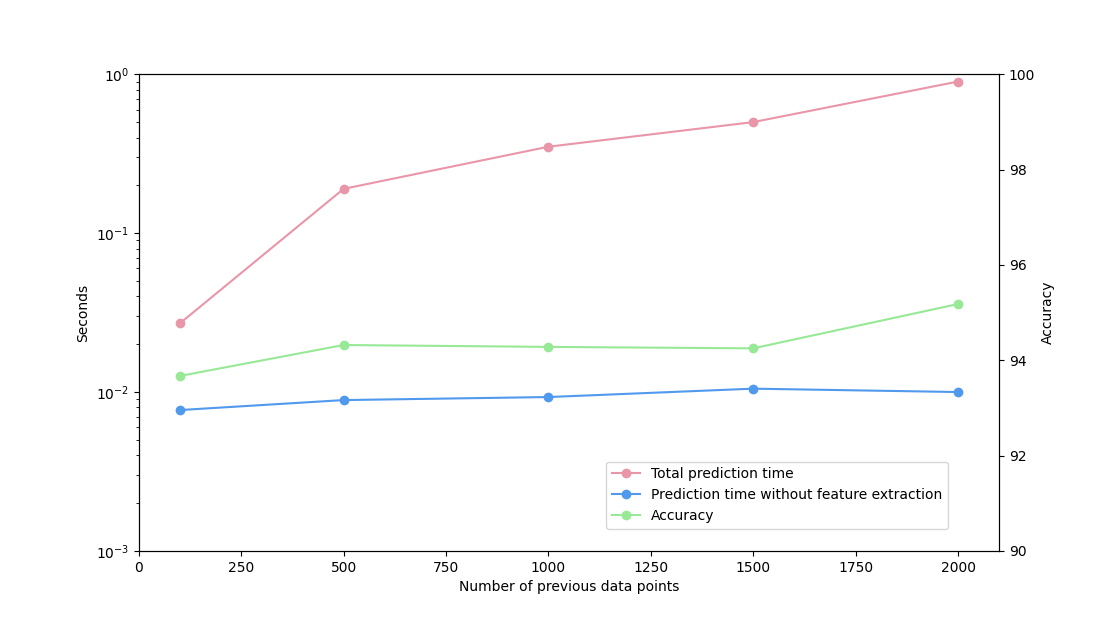
\includegraphics[width=\textwidth]{figures/speed_per_dp_count.png}
	\caption{Execution speed and score versus number of previous data points}
	\label{fig:speed_per_dp_count}
\end{figure}

The measured data shows that by only considering $100$ previous data points the total prediction time can be reduced to $27ms$ with a corresponding accuracy of $93.67\%$ compared to $900ms$ and $95.15\%$ ($2000$ previous data points). Reducing the amount of data points below $100$ yielded very low accuracies ($<80$) while not reducing the prediction time significantly. Compared to the average response times of all the experiments' requests of $23.78ms$ and $16.67ms$, this is still a very significant amount. One method which might be acceptable is to run the prediction in parallel to the request processing and waiting a few milliseconds for the result before returning a response. Another method would be to separate the feature extraction from the combination of data points. But for some values this might not be possible or lose information, e.g. mean or standard deiviation of several data.
A better method might be to separate the prediction system entirely from single requests and decide on a per-user basis asynchronously after enough samples have been collected whether to take any action against it or not.




\chapter{Discussion}
In the context of bot detection and the web in general, the method of attack and type of target(-website) can vary significantly and are changing constantly. This is one of the reasons that web security is an ongoing cat and mouse game and represents a practically unsolvable problem with many unkowns. This work needs to make many assumptions in order to limit the scope and produce generalizable data.

One limitation is that this approach does only work for clients that use a pointer device, i.e. mouse, touchpad or touch screen. If this is not acceptable, a different method would additionally need to be used. This applies for example when screen readers, text-based browsers or automated clients should be supported. A compromise might be to use the pointer-based system to trigger additional security checks at critical actions, such as registering an account or posting content.

Another problem might be that this approach does not elimitate all user tracking and the associated data processing. Especially public pages that should to be accessed without the need to ask for explicit confirmation. Although this is a general problem for websites that store or process user data, e.g. in the form of cookies, it applies to this approach as well. The main advantage is that the proposed system can be run by the same operator and does not need to send user data to any third parties.

Even the best-case accuracy of $>99\%$ might be not enough for some applications, especially if critical decisions depend on the system.

\chapter{Conclusion}

The Evaluation shows that in general a bot detection system which incorporates pointer data can be considered for practical use. Its main performance criteria in the form of high accuracy and a low false positive rate are given but its actual value is dependend on the concrete usage and operation.

The requirement to be privacy-friendly is met by using a machine-learning-based system which can be deployed by operators themselves and does not need to share any identifiable user data with third parties.

Finally, good execution speed is not achieved in every case and does degrade the overall value of the proposed system. In practice, higher accuracy can be traded for higher execution speed. Additionally the system has many possibilities to be optimized and improved which would meet this requirement as well.

\begin{raggedright}
  \printbibliography
\end{raggedright}

% Appendix
\chapter*{Appendix}

\section*{Source Code}

\begin{itemize}
	\item Experiment Websites and Machine Learning Model: Github repository\footnote{\url{https://github.com/timesqueezer/fmexp}} and attached USB drive
	\item Thesis: Github repository\footnote{\url{https://github.com/timesqueezer/uni/thesis}}
\end{itemize}

\end{document}
